In order to find the 3D map of the target, we use the triangulation method seen in the previous section on a grid of lighting points. To do so, for each lighting point, we have to use two different angles $\bm{\alpha}$ and $\bm{\beta}$. Previously, $\bm{\alpha}$ was the angle between the focal axis of the camera and the beam but now it is the angle between the focal axis of the camera and the beam projected on the plane y=0 and $\bm{\beta}$ is the angle between the focal axis of the camera and the beam projected on the plane x=0 (see figure \ref{3dmap}). In the same way, the distance \emph{d} camera-artificial light of source becomes $\bm{d_x}$ and $\bm{d_y}$.

\begin{figure}[H]
  %\centering
  \centerline{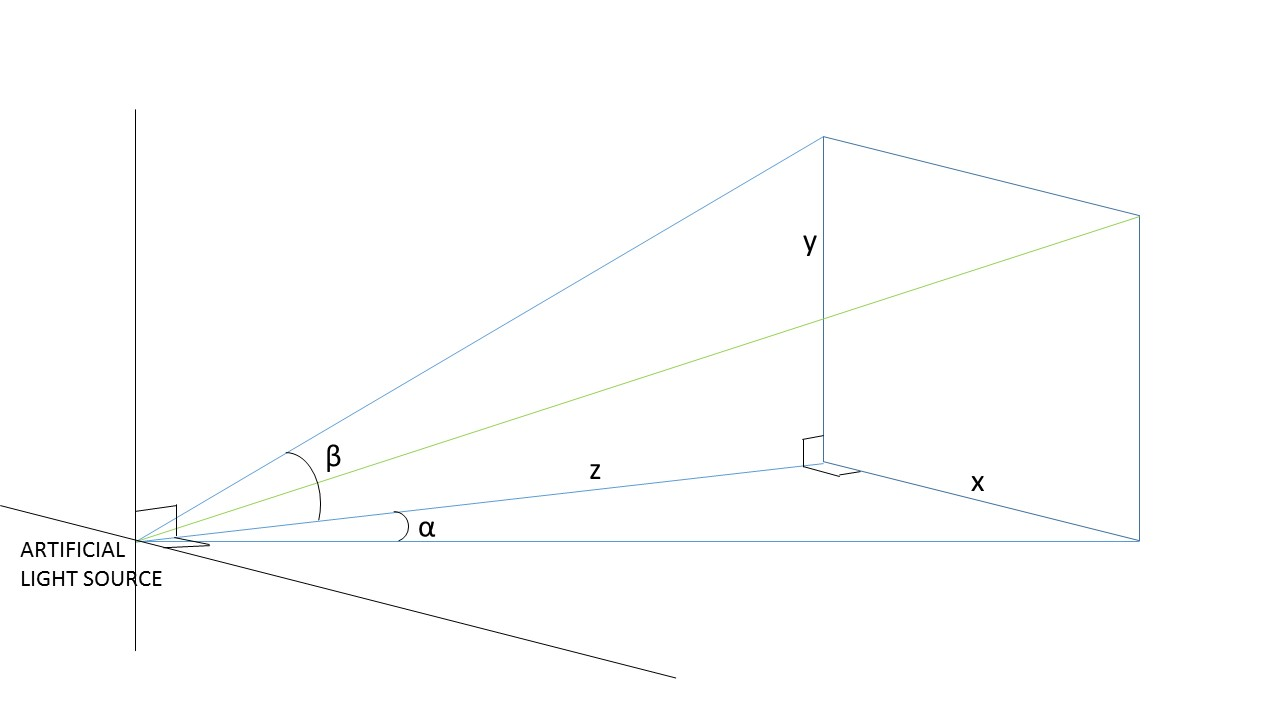
\includegraphics[scale=0.4]{fig/3dmap.jpg}}
  \caption{schema of a beam of the artificial light source}
  \label{fig:3dmap}
\end{figure}

Thus, the new distance camera-target is

\begin{equation}
z = \frac{d_x}{p_{pixels,x}\frac{P_{size}}{f_0}+ \tan \alpha}
\label{eq:formule3D}
\end{equation}

Then, to find the (x,y) coordinates of the point, we have

\begin{align}
x & = z \tan \alpha - d_x \\
y & = z \tan \beta - d_y
\end{align}

We subtract $d_x$ and $d_y$ in order to change from the artificial light source system of axis to the camera system of axis.